\documentclass{article}
\usepackage{longtable}
\usepackage{graphicx}
\usepackage{booktabs}% http://ctan.org/pkg/booktabs
\usepackage{xcolor}
\newcommand{\tabitem}{~~\llap{\textbullet}~~}
\newcommand\mytodo[1]{\textcolor{red}{#1}}
\usepackage{array}
\usepackage[style=numeric,backend=bibtex,sorting=none]{biblatex}
\usepackage{caption}
\usepackage{amsmath}
\usepackage[british]{babel}
\usepackage{a4wide}

\bibliography{Fragestellung}

\begin{document}
\begin{large}

\title{Extending prediction of parking occupancy to untracked city areas using city background information}
\maketitle

\section{Abstract} 
Several smart cities around the world have begun monitoring parking areas in order to predict free spots and help drivers that are looking for parking. The current results are indeed promising, however this approach is limited by the high cost of sensors that need to be installed throughout the city in order to achieve an accurate prediction rate. This work in\-ves\-ti\-gates the extension of forecasted parking information from areas equipped with sensors to areas that are mis\-sing them. To this end, si\-mi\-la\-ri\-ty va\-lues between city neighborhoods will be computed based on background data, e.g. from geographic information systems. Using the derived si\-mi\-la\-ri\-ty va\-lues, the adaptation of occupancy rates from monitored- to unmonitored parking areas will be analysed.

\section{Technical details}
\subsection{Data}
There are some cities around the world that offer open parking occupancy information, either for a time interval in the past and/or currently. In Europe, the author found Dresden\cite{dresden}, Zurich\cite{zurich} and Cologne\cite{cologne} up to now that offer this kind of information for car parks. In the US such data is found for the cities of Philadelphia\cite{philly}, Santa Monica\cite{monica} and San Francisco\cite{sfpark}. 

The SFpark project in San Francisco offers a large dataset for on-street parking. Occupancy data has been collected there for over two years between April 2011 - July 2013 in more than 400 blocks, resulting in over 1 million data records. The project was conducted with the main purpose of leveling off the parking occupancy in the city. In seven pilot areas of the city parking prices were adapted to the level of occupancy. Therefore drivers received incentives to park in areas less occupied by paying a smaller parking fee. Another two control areas were used to verify the effectiveness of the pricing measures. Parking data for all nine areas exist (see figure~\ref{fig:sfpark_areas}). In the following, SFpark will be taken as data reference.

\begin{figure}[!ht]
    \centering
    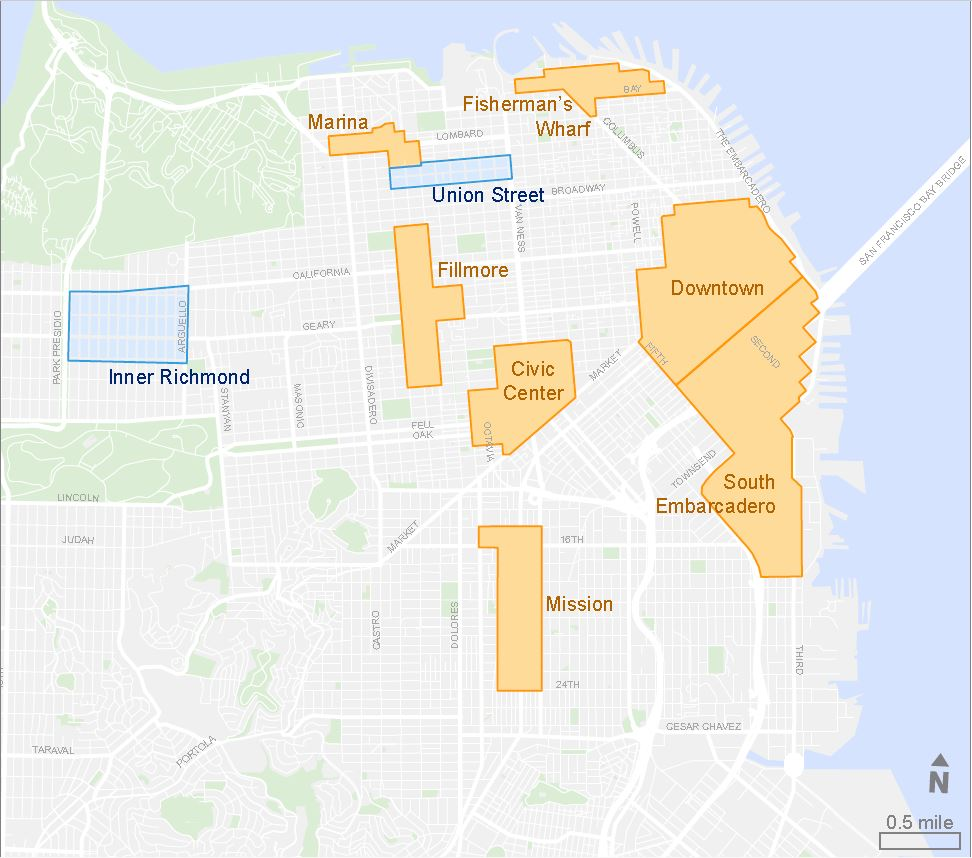
\includegraphics[width=0.7\textwidth]{sfpark_areas.jpg}
    \caption{SFpark pilot and control areas}
    \label{fig:sfpark_areas}
\end{figure}

\subsection{City background information} 
Metadata that indirectly indicates parking demand is highly interesting to analyse. Do areas with a high number of restaurants display a similar parking occupancy graph? Can parking behavior for quarters with a high sales revenue be correctly guessed?

Some of this metadata can be found in geographic information systems. In OpenStreetMap there can be found a large number of Points of Interest (POIs) that mark buildings of various types (offices, restaurants, cinemas, etc.) and some of their properties (working hours, opening times, capacity, etc.). Moreover, the physical coordinates corresponding to POIs are accessible as polygons, while streets are represented as lines. Hence further data can be inferred when merged with street metadata, e.g. size of parking lane in front of an office. This information will be used to create a "profile" of an area. For example, the POIs in northern part of San Francisco are displayed in figure~\ref{fig:available_gis_data}. 

\begin{figure}[!ht]
    \centering
    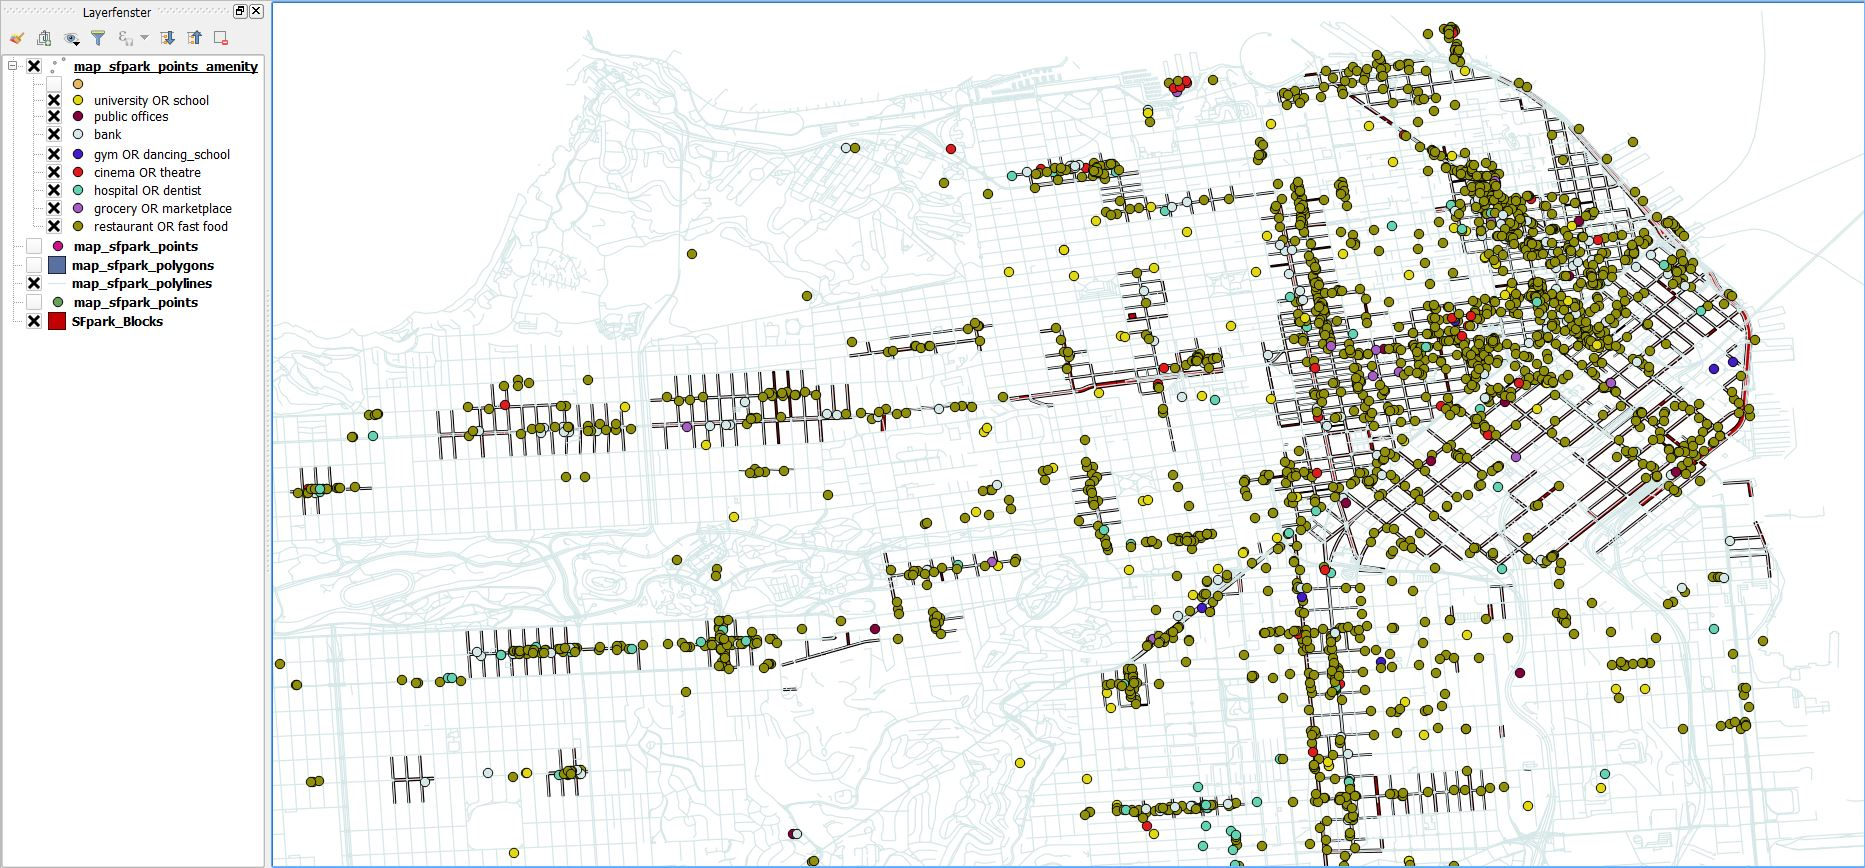
\includegraphics[width=\textwidth]{available_gis_data.png}
    \caption{Screenshot from QGIS showing the dimensions of metadata available in OSM}
    \label{fig:available_gis_data}
\end{figure}

Additionally, SFpark provides sales revenue information for its original nine areas, concerning food product and general retail. Even some of the information that the ML model is trained with but has little added value there can be used to consolidate an area profile. 

\subsection{Method} 
\begin{enumerate}
\item \textbf{Cluster all blocks into compact areas}

Parking information is initially provided per block face. A block is the space between two consecutive streets in a typical American city (see figure~\ref{fig:block_faces}). Since blocks are too small and unrepresentative a unit to process data for, the first step will be to geographically cluster blocks.
A method as K-Means, K-Medoid or similar will therefore be used to group individual block faces into a convenient number of clusters. Only the geographic position and (Euclidean/Manhattan) distance are needed for clustering. Monitored and unmonitored areas will be clustered separately.

\begin{figure}[!ht]
    \centering
    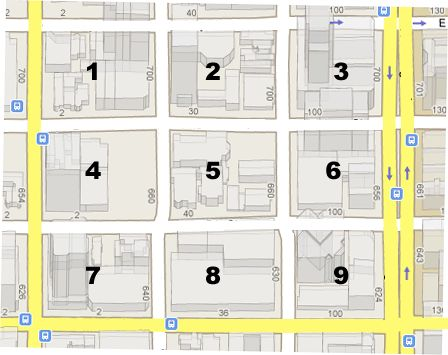
\includegraphics[width=3.0in]{blocks.jpg}
    \caption{Blocks in a city, with each block displaying four faces for each surrounding street\cite{blocks_source}}
    \label{fig:block_faces}
\end{figure}

\item \textbf{Calculate pairwise similarity between unmonitored- and monitored clusters}

Per cluster, vectors with the following dimensions will be built using GIS attributes:
\begin{itemize}
\item count of office buildings $\times$ their capacity/size
\item count of cinemas/theaters/concert halls $\times$ their capacity/size
\item count of restaurants/fast food $\times$ their capacity/size
\item (other types of buildings that create parking demand)
\end{itemize}

Further attributes that account for parking demand may be added to this list. The degree in which attributes increase or decrease the similarity of vectors will be evaluated.

A similarity measure is introduced at this point. Candidates are Cosine Similarity, Jaccard Index, Kullbach-Leibler Divergence, possibly after reducing data dimensionality by running Principal Component Analysis or Latent Semantic Analysis. 

Taking Cosine Similarity as an example, between vectors $A$ and $B$ with $n$ dimensions, it is defined as:
$$ \text{similarity}(A,B) = \frac{A \cdot B}{||A|| \cdot ||B||} = \frac{\sum_{i=1}^{n}A_iB_i}{\sqrt{\sum_{i=1}^{n}A_i^2} \cdot \sqrt{\sum_{i=1}^{n}B_i^2}}$$
Its value lies generally between $-1$ and $1$, but in our case it is limited to $[0..1]$, since all dimensions have positive magnitudes. $0$ corresponds to uncorrelated vectors, while $1$ indicates that the vectors are the same.

\item \textbf{Build prediction models for monitored clusters}

For training ML models, the following SFpark attributes will be used:
\begin{itemize}
\item parking price - varies with zones and block faces
\item traffic density - determined by sensors installed on the street surface, it indicates how much from a street section is occupied by cars
\item fuel price - daily rate, valid for the whole city
\item precipitation - the amount of rain or snow that fell per day, valid for the entire city
\item street closing information - due to street parades, construction work, etc.
\item parking demand up - signals the block faces that have a higher parking demand at a certain point, due to concerts or other extraordinary events
\item construction site - signaled for a block face that it affects
\item parking place count - the number of operable parking spots
\item occupancy - the rate of occupied spots divided by the parking place count
\end{itemize}
The target variable for the model is $occupancy$. 

The prediction mo\-dels will be computed using state-of-art methods, like neural networks, autoregression models and support vector regression\cite{chen}\cite{rajabioun}.

In figure~\ref{fig:training_data} there is a snippet of training data. 

\begin{figure}[!ht]
    \centering
    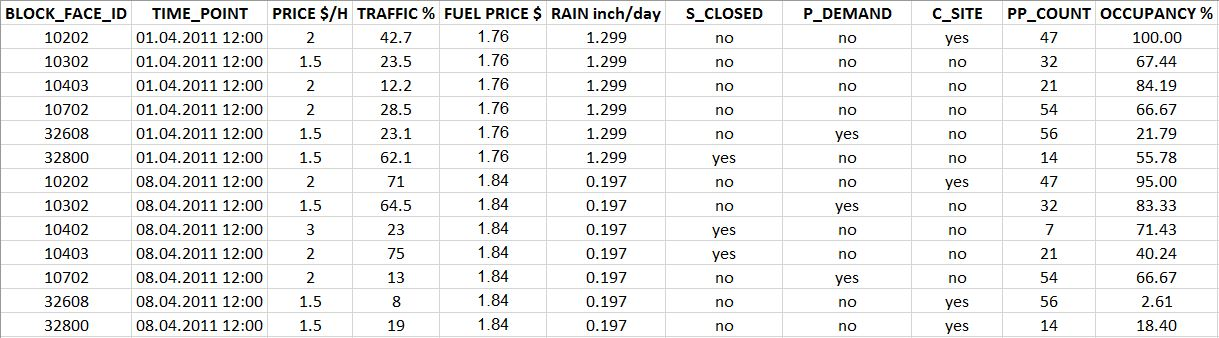
\includegraphics[width=\textwidth]{training_data_snippet.jpg}
    \caption{Training data snippet indicating SFpark attributes}
    \label{fig:training_data}
\end{figure}

\item \textbf{Apply prediction models to unmonitored clusters, factoring in the respective similarity value}

For every unmonitored cluster $C_u$:
\begin{enumerate}
\item the monitored cluster $C_m$ will be selected that has the maximum similarity between the two clusters
$$ S = max\{similarity(C_u,C_m)\}, \forall C_m \in \mathcal{C} $$
\item $C_m$'s model will be applied on the SFpark attributes of $C_u$, resulting in the prediction
$$ P = M_{C_m}(attr) $$
\item the final result will be a value interval
$$ \text{occupancy}(C_u,\text{attr}) = [max\{0, P-(1-S) \cdot 100\},min\{100, P+(1-S) \cdot 100\}] $$
\item in case the resulting interval is too large, the previous steps can be repeated for the next most similar cluster $C'_m$. By calculating the respective interval and intersecting all of them, one may arrive at a more precise result.
\end{enumerate}
\end{enumerate}

\subsection{Evaluation} 
In order to verify the hypothesis that parking occupancy in unmonitored areas is up to a degree similar to the occupancy in some monitored areas, concrete data is needed for the respective sensor-free locations. We will therefore split the sensor data available and take into consideration only areas for which occupancy data exists.

To test the accuracy of the inferred occupancy va\-lues, we estimate to need 10\% of the available data. Training will therefore be performed using the remaining 90\%.


\subsection{Originality of work} Up to now, the smart parking literature concentrates on capturing data and predicting parking information using static or mobile sensors, by covering the areas for which future rates are calculated\cite{lin}. An extrapolation approach as described here, to the best of my knowledge, has not been explored yet.

\end{large}

\nocite{*}

\printbibliography

\end{document}